\section{Architecture}
\label{sec:Architecture}
% Owner: Jani
% Reviewed: Johanna
%
Confronted with the challenge of creating a high-performance and expandable infrastructure for simulating a marketplace with different merchants and consumers, a microservice architecture was created allowing the user to scale, exchange or add single service ad-hoc and on demand. Each service within our architecture implements one business artifact. This architecture pattern comes with the cost of a communication overhead and requires farsighted API design.\\

Figure~\ref{fig:fmc} describes the underlying architecture modeling as FMC\footnote{\url{http://www.fmc-modeling.org/}} diagram. We understand a single realization of this architecture as one simulation universe, meaning that key components are meant to be unique in this universe. 

When initiating a new simulation universe, it comes along with the marketplace component, as well as the producer-component and a management UI for controlling each service. While the producer offers products, the marketplace holds the current market situation and handles price updates and purchases of goods. Each transaction handled by the producer and marketplace is logged to a stream database, namely Apache Kafka\footnote{\url{https://kafka.apache.org/}}. Further, those logs are being analyzed and aggregated through a batch data processing component which is in our case Apache Flink\footnote{\url{https://flink.apache.org/}} and written back into a new Kafka topic. Those details, then, can be accessed through a socket connection or REST interface provided by a kafka-reverse-proxy. 
\todo[inline]{are it really five?} 
To liven the place up, numerous consumers or merchants may join and participate in this market simulation. By default, one consumer and five merchants are deployed with already implemented strategy. Those behaviors are deepened in chapter \ref{sec:Behaviors} while the choreography of the single services is delineated in chapter \ref{sec:Choreography}.

%
\begin{figure}[h]
    \centering
    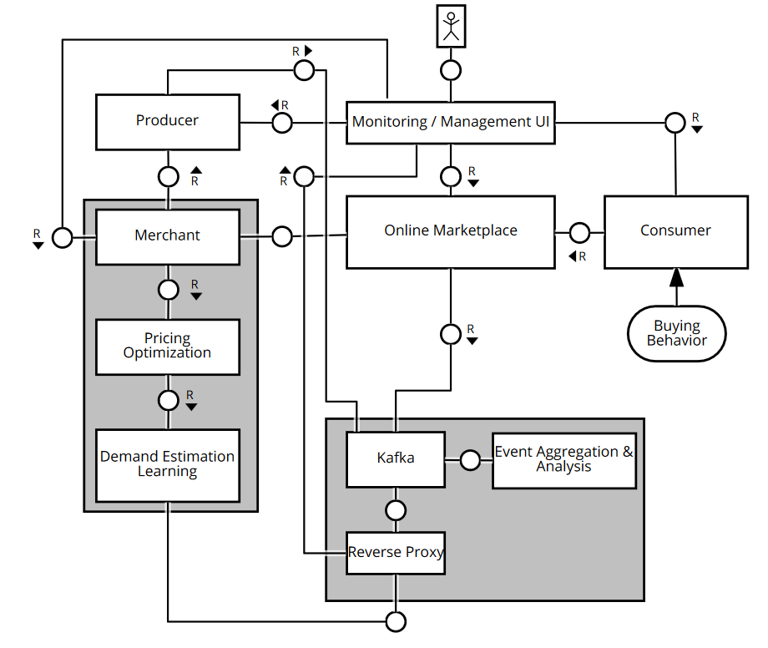
\includegraphics[width=0.5\textwidth]{images/architecture_fmc.png}
    \caption{FMC diagram of the Price Wars architecture}
    \label{fig:fmc}
\end{figure}
%